The experiment was run at the National Superconducting Cyclotron Laboratory (NSCL) in East Lansing, Michigan. 
The experiment was run from September 1, 2015 to September 7, 2015.

\section{Experimental technique}
The technique used was a calorimetric technique, where the isotope of interest is implanted inside a detector.
This reduced several effects could otherwise distort the beta decay spectrum.
The largest of these is backscattering.
If a beta decay source is placed outside a scintillator, there is a chance that the electrons will go into the detector material and bounce back out.
This happens in the surface of the detector, and therefor the electron deposits very little energy into the detector. 
Backscattering causes the largest distortion at low energies.
However, the description of backscattering using detector simulations varies too much to get a sufficient description for a precision shape measurement \cite{Huy18}.
Beta decay electrons cans scatter out of the sides of the detectors as well. 
This also distorts the beta spectrum in a different fashion. 
Lastly if there is a dead layer at the surface of the crystal, the energy deposited in that layer will not be absorbed.

With the calorimetric technique, the radioactive nucleus is surrounded by detector material.
As long as the nuclei are implanted deep enough, the electrons will not have enough energy to escape the detector.
Even if the electron scatters several times, it still deposits all it's energy.
This range depends on the detector material.
Since any dead layers are at the surface, the decays inside the detector do not see them.
A $4\pi$ angular coverage is also obtained, as the detector material surrounds the source.

There are some caveats for a calorimetric technique. 
The first is that a large enough detector is needed.
Otherwise the electrons could escape at high energies.
This means that this technique works best with scintillator detectors, since it is hard to grow semi-conductor detectors large enough to absorb all the electron energy.  
A large effect is that electrons moving through the detector material will emit a lot of bremsstrahlung.
Using a low-Z detector material will lessen this effect.
However, Monte Carlo detector simulations can describe the production and absorption of bremsstrahlung to enough precision to allow for a precision beta decay measurement. 
Another issue is that accelerators used to generate the isotope of interest must be able to create them at high enough energy in order to implant the isotopes deep enough into your detector.
This limits what nuclei can be used for this technique.
The act of implanting the nuclei gives the detector a lot of energy. 
This means that an implant and decay cycle is need for this experimental technique.

For this experiment, a  beam of  $^{20}$F, was implanted into two different detectors, which were used to cross-check different systematic effects.
One was a CsI(Na) scintillator detector, and the other was a  EJ-200 polyvinyltoluene scintillator detector. 
After an amount of $^{20}$F was implanted, the beam was turned off by dephasing the RF that drove the cyclotrons.
Then, the $^{20}$F was allowed to decay inside the detector. 
Given the half-life of $^{20}$F of 11 s, the measuring time was varied between 22 and 60 s.

\section{Creating $^{20}$F Beam}

The beam of $^{20}$F was created at the coupled cyclotron facility at the NSCL.
The primary beam of $^{22}$Ne was accelerated by the coupled cyclotrons to 150 MeV/A. 
A typical intensity of the primary beam was around $60 * 10^{-5}$pnA.
It was impinged on a 188 $\frac{mg}{cm^{2}}$ Be target and sent through the A1900 fragment separator. 
The resulting $^{20}$F beam was at an energy of 130 MeV/A. 
The intensity of the $^{20}$F was about $2 * 10^{-5}$ pnA.
The beam was sent to the experimental vault were the detectors were sitting.
\subsection{Beam Purity}

The purity measured there was at 99.4\%, with the main contaminates being  $^{19}$O. 
This was measured up stream of the detector set up.
To double check the beam purity, two detectors were used. 
One was a thin Si PIN detector that was used as a sectionE detector. 
The other detector was a small CsI(Na) detector similar to the implant detector that was used during the steering and during the beam size measurement. 
It had a much lower voltage than the one used for the implantation measurement. 
Both of these in tandem were used to build a particle identification plot.
From this, it was found that the beam is very clean.

\subsection{Beam Size and Location}
To test the size of the beam, a parallel plate avalanche counter (PPAC) was used.
The size of the detector was 10 cm by 10 cm square. 
It was placed 65 cm upstream of the target.
A horizontal and vertical grid was in the detector.
Depending on where on each of the grids the particles hit, different charges were sent to either end of the PPAC.
The signals were fed into a digital data acquisition system, and read out as an energy.
The difference of the two signals divided by the sum was interpreted as a position.

To calibrate the PPAC , a mask with several holes was used. 
This mask covered the front of the detector, and an alpha decay source in the vacuum was placed in front of the PPAC.
Then, everything was left to run until an image of the mask was formed.
The mask had holes in it every 1 cm. 
It also had a large L shaped hole so that the orientation of the mask could be seen. 
With this, the PPAC could be calibrated.

Before taking data for the beta decay spectrum measurement, the PPAC was inserted into the beam.
After adjusting the parameters of the upstream beam optics, the final beam size at the PPAC was measured.
The calibrated data of the signals was built into a 3-D histogram.
There was some ringing in the PPAC, so the peak of the beam spot was fitted with a 3-D gaussian function.
The average of the Gaussian and the sigma in the x and y direction was taken. 
From the sigmas, the half widths at half maximum (HWHM) in both directions were calculated. 
The distribution of the locations were sampled at eight different points. 
The points are shown as the black dots in Fig: \ref{fig:PPACSpotch}.
They are one HWHM away from the center. 

\begin{figure}
	\centerline{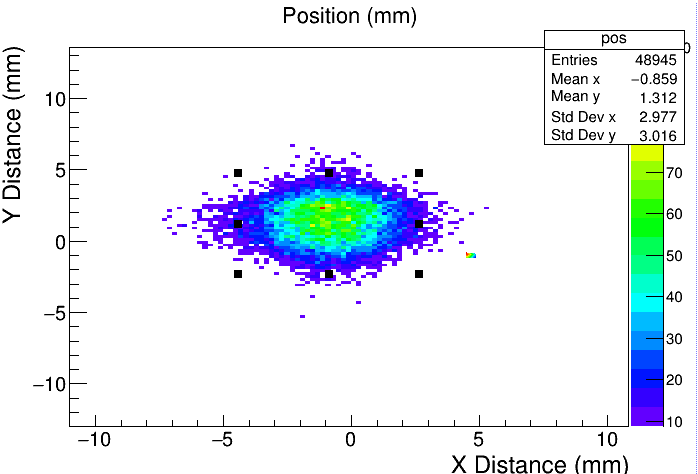
\includegraphics[width=0.88\textwidth]{PPACFitted.png}}
	\caption{The beam spot of the calibrated PPAC spectrum. 
		 The samples of the spectrum that were averaged together are shown in the black dots.
		 The center of the fit is not shown.}
	\label{fig:PPACSpotch}
\end{figure}  

After averaging the 8 points, the range on the z axis was taken from the average of those points to the top.
The resulting beam was measured to be 8 mm by 6 mm large.

This is the size of the spot at the PPAC. 
Ion optics simulations were used to build the cross section of the beam at the PPAC and at the target.
Using these cross sections, the magnification between the two locations was calculated.
The magnification was different between the x and y directions.

For the depth of the implantation of the beam, ion simulations were used. 
The LISE++ program was fed the beam meagnets. It was given the energy of the beam and the detector set up. 
It then calculated the depth of the implantation of the detector and the range of the depth inside the detector. 
This gave a depth of 3.02 cm in side the PVT detector and a depth of 1.156 cm in the CsI(Na) detector. 
The range of the depth was 1.2 mm in the PVT detector and 0.4 mm in the CsI(Na) detector.

\subsubsection{Verifcation of Implant Depth}

In order to verify the simulations for the beam implant depth, a degrader was inserted into the beam for a beam depth measurement.
The degrader was made of aluminum and had two different thicknesses: 7.89 mm and 11.38 mm. 
The beam was caught by a CsI(Na) scintillator of a similar design to the one used for the implantation measurement.The angle of the degrader was changed to change the ective thickness of aluminum that the beam
had to travel through. By varying this thickness to the one predicted to stop the beam out side of the detector, the depth of implantation could be verified. 
This was done after the main run, and the simulations proved to be correct.

\section{Detector Configuration}

\subsection{$^{20}$F Decay Detectors}
One implant detector was a scintillator 3 in diameter by 3 in long cylinder of EJ-200 polyvinyltoluene (PVT).
It was attached to a clear plastic disk attached to a photomultiplier tube.
The idea was to avoid a rate dependent gain effect that was seen in a previous experiment.
The plastic detector signal is fast (around 100 ns) which makes pile-up a lesser concern.
This detector was built by collaborators for this experiment.
During the experiment the voltage on the PMT of this scintillator was varied.
This was due do an observed distortion in the beta decay spectrum.
A gain monitoring system was installed.

To monitor the gain of the plastic detector, a plastic disk containing an optical fiber was placed between the crystal and the photomultiplier tube. 
The other end of the fiber was fed into a box with an LED driven by a function generator, which ran at a trigger rate of 500 counts per second. 
The function generator produced two pulses separated by 136 $\mu$s.
These two pulses had different amplitudes, so that the gain drift could be monitored by observing the drift from two different energies.
The box was made light-tight with electrical tape and black paint.
An additional optical fiber fed the light to a Si PIN diode.
This was to monitor the light output of the LED.

To help check for systematics effects, another implant detector was used.
It was a 2 in by 2 in by 4 in  CsI(Na) detector. 
This detector was a module from the CAESAR array \cite{Wei10}.
It does not have any gain monitoring like the PVT detector, but it is similar to a detector used in a different experiment. 
The other experiment was a similar measurement with $^{6}$He instead of $^{20}$F.

In order to measure the gamma ray from the $^{20}$F decay, a frame was built to hold four cubic 3 in CsI(Na) detectors.  
These were also part of the CAESAR array.
The frame to hold the four detectors was designed to be able to move the four outer detectors around in various configurations.
However, no other configurations were used during the experiment. 

A sketch of both detector configurations is shown in Figure \ref{fig:detsketch}.

\begin{figure}
	\centerline{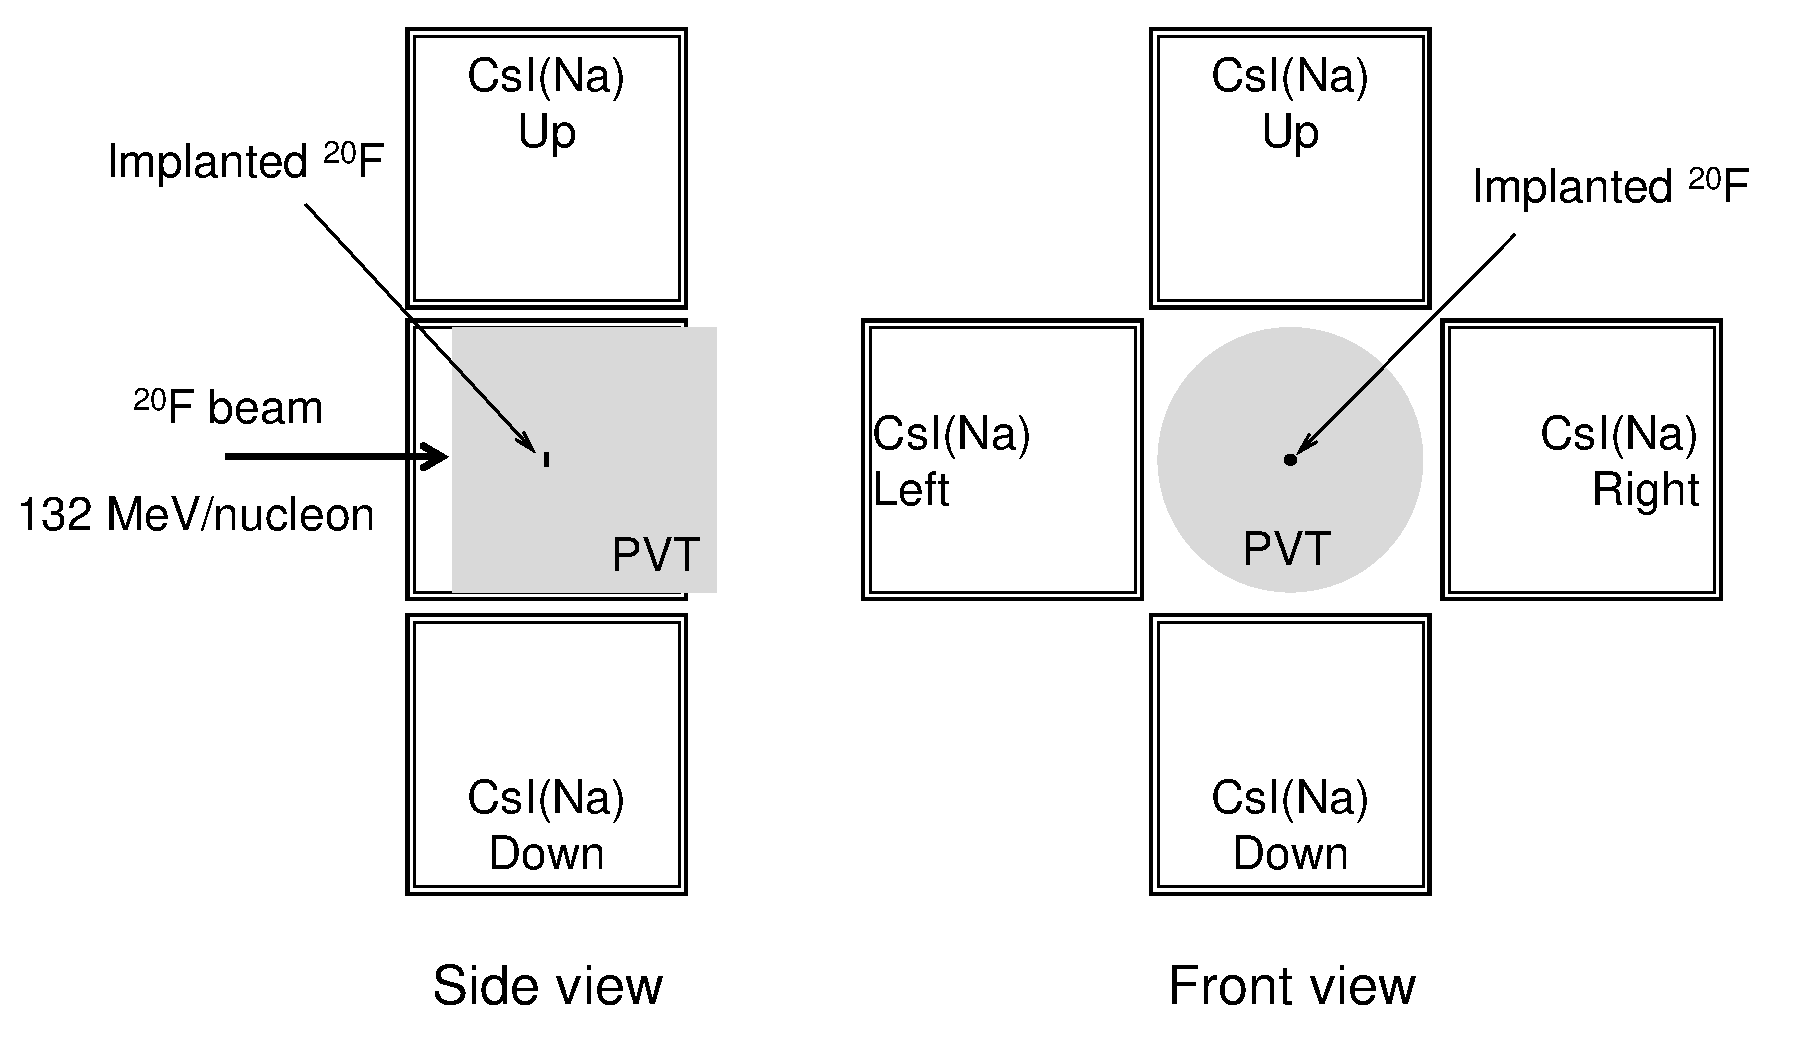
\includegraphics[width=0.68\textwidth]{fig_setup.pdf}}
	\caption{A sketch of the detector set up. 
	Shown here is with the PVT detector implant.
	The CsI (Na) detector was centered in the middle of the the four gamma detectors and recessed by 1 inch.
	The bottom image shows a side of the detector set-up.}
	\label{fig:detsketch}
\end{figure}

To switch between different implant detectors, the central detector in the frame was removed and put on the floor.
The other detector was placed in the center of the four gamma detectors.
The PVT detector was supported on a metal rail, while the CsI (Na) detector was supported on pile of scrap aluminum.
The rail for the PVT detector, along with the four gamma detectors,  can be see in figure \ref{fig:PVTPicture}.

\begin{figure}
	\centerline{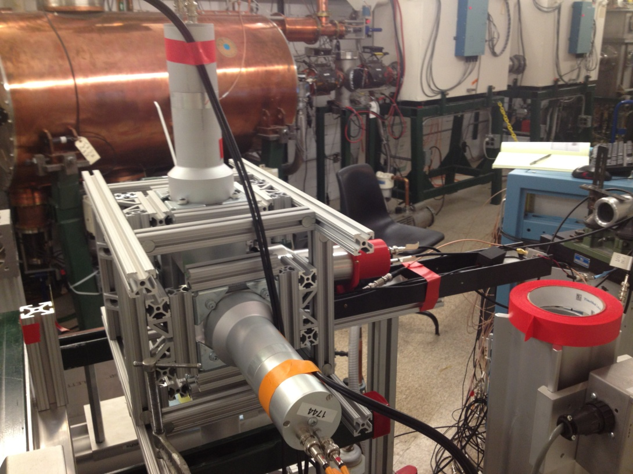
\includegraphics[width=0.68\textwidth]{fig_PVTSetupPicture.png}}
	\caption{A piture of the PVT configuration. 
		 The colored tape on the PMTs of the gamma detectors was to keep track of what power and signal cable went to which detector.
		 The rail the detector rested on can be seen.
		 The optical fibers (the black cords) can be seen running into the black box with the LED.
		 }
	\label{fig:PVTPicture}
\end{figure}

A better view of the gamma detector cross can be seen in figure \ref{fig:CsIPicture}.
\begin{figure}
	\centerline{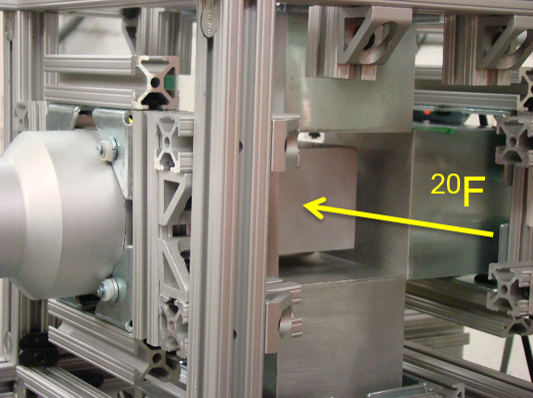
\includegraphics[width=0.68\textwidth]{fig_CsISetupPicture.png}}
	\caption{A piture of the CsI setup.
		 The active cyrstal of the implant detector can been seen much better. 
		 }
	\label{fig:CsIPicture}
\end{figure}

\subsection{Detector Frame}
The aluminum sheathing came with the detectors.
However, the bars of aluminum in figure \ref{fig:PVTPicture} were not part of the detector array.
These bars made up the frame which was designed seperately.
In order to design the frame, the program FreeCAD was used.
The detector crystals were modelled as cubes. 
The frame was made from extruded aluminum alloy bars from 80/20 Inc.
Models of the bars were positioned in the program, and the frame built up from there.
The frame was designed so that the gamma detectors could move around into a pin-wheel configuration.
This configuration was not used during the experiment.

\subsection{Powering the Detectors}

To power the gamma and implant scintillators, 3 2-channel NHQ 212M ISEG power supplies were used.
The Si detector was powered by a Tennelec TC248 amplifier.
The PPAC was powered by an integrated power supply.

Each detector had a different voltage. 
The PVT implant detector was varied in voltage over the course of the experiment.
This was due to concerns about saturation effects.
Initially, the high voltage on the PVT detector was chosen to take advantage of the dynamic range of the detector.
For the PPAC, 
The voltage for the four gamma detectors was chosen so that they had roughly the same gain.
The voltages of the detectors is shown in table \ref{tab:detvolt}.
\begin{table}[!hbt]
	\centering
		\begin{tabular}{l|r}
		Detector & Power Supply Setting (V) \\ \hline
		PVT Implant (Sets 1-4) & -975 \\
		PVT Implant (Set 5) & -856 \\
		PVT Implant (Set 6) & -780 \\
		CsI (Na) Implant & 780 \\ 
		CsI (Na) Gamma 1 & 930 \\
		CsI (Na) Gamma 2 & 1000 \\
		CsI (Na) Gamma 3 & 970 \\
		CsI (Na) Gamma 4 & 1015 \\
		Si Pin & 20 \\
		Pin diode & 15 \\
		PPAC & 560  
		
		\label{tab:detvolt}
		\end{tabular}
\end{table}

During the implantation cycle, a large amount of current was generated in the implant detectors.
In order to counteract this, a limiter box was installed for the PVT detector for sets 3 to 6.
The limiter box had several relays that cut the power to the PVT detector's photomultiplier tube during the beam on cycle. 
To accomplish this, the limiter box was given the same signal that fed the beam on/beam off for the cyclotrons.
Due to concerns about the beta decay spectrum shape, the voltage on the PVT detector was changed as the experiment went on. 
For the CsI(Na) implant detector, the HV supply had the current limiter enabled.
The power setting was not changed for the CsI(Na) implant detector. 


\section{Experimental Conditions}
The data was taken in runs of roughly one hour. 
However, many runs where cut short when the DAQ stopped recording data for one of the detectors.
This was usually the up gamma detector, and was correlated with the start of a new implant cycle.
In order to properly measure the decay, the beam was pulsed with an implantation time of anywhere from 1 to 2 seconds, and a decay time ranging from 22 s to 32 s. 
The beam was turned off since the light from the implantation of the beam would drown out any signal obtained. 
A run with a decay time of 60 seconds was also taken for each implant detector. 

To achieve the beam pulsing, two timer boxes were used.
A CAEN N1145 quad scaler module was used to control the beam off time.
This module had a digital control of time down to 1 ms.
Once the the time finished counting down, a signal was sent to a second module. 
A CAEN N93B dual timer used the signal from the quad scaler as a start signal.
The time period was set using a dial, which was less precise. 
Once the dual timer finished its time, it sent a signal back to the quad scaler to restart the cycle.
The output of these two modules created a signal with one voltage level during the dual timer's time and another voltage condition during the quad scaler's time.
This signal was fed into a box.
The voltage level during the quad scaler's time dephased the cyclotron RF, turning the beam off.
When the dual timer voltage level occurred, the RF returned to the tuned value, turning the beam on.  


